\chapter*{Proposition 6}
\label{prop:6}

\begin{figure*}[ht]
    \begin{center}
    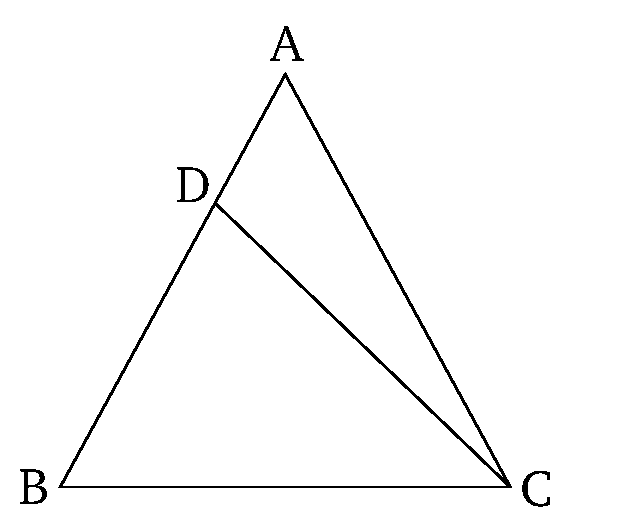
\includegraphics[width=0.5\linewidth]{figures/fig06e.eps}
    \label{fig:prop_6}
    \end{center}
\end{figure*}

If a triangle has two angles equal to one another then the sides subtending the
equal angles will also be equal to one another.

Let $ABC$ be a triangle having the angle $ABC$ equal to the angle $ACB$. I say that
side $AB$ is also equal to side $AC$.

For if $AB$ is unequal to $AC$ then one of them is greater. Let $AB$ be greater. And
let $DB$, equal to the lesser $AC$, have been cut off from the greater $AB$ [Prop.~1.3].  And
let $DC$ have been joined [Post.~\ref{post:1}].

Therefore, since $DB$ is equal to $AC$, and $BC$ (is) common, the two sides $DB$, $BC$ are equal to the two sides $AC$, $CB$, respectively, and the angle $DBC$
is equal to the angle $ACB$. Thus, the base $DC$ is equal to the base
$AB$, and the triangle $DBC$ will be equal to the triangle $ACB$ [Prop.~1.4], the lesser
to the greater. The very notion (is) absurd [C.N.~\ref{cn:5}]. Thus, $AB$ is not unequal
to $AC$. Thus, (it is) equal.

Thus, if a triangle has two angles equal to one another then the sides subtending the
equal angles will also be equal to one another. (Which is) the very thing it was required to show.


\section*{Commentary}

\begin{proposition}\label{proposition_6}\lean{Elements.Book1.proposition_6}\leanok
    In $\triangle ABC$, if $\angle~ABC = \angle~ACB$, then $|AB| = |AC|$.
\end{proposition}
\begin{proof}
    \uses{proposition_3,proposition_4}\leanok
    See the original proof by Euclid.
\end{proof}
